\section{Aplicación del sistema BCI}
\label{sec:aplicacionBCI}

Con el objetivo de facilitar el uso del EEG e integrar todas las utilidades del sistema BCI, se ha desarrollado una aplicación que constituye el punto de entrada a todas las funcionalidades del sistema: desde la configuración del hardware del EEG, la evaluación de calidad de señal y la visualización de grabaciones, hasta la ejecución de experimentos y la evaluación de los sujetos. Funciona mediante una interfaz de línea de comandos y su diseño modular permite ejecutar de forma independiente cada uno de los módulos que componen el sistema.

El desarrollo de esta aplicación ha simplificado significativamente la realización de grabaciones, experimentos y ajustes de configuración, convirtiéndose en una solución a medida de las necesidades del proyecto. Si bien la aplicación oficial de BrainAccess ofrecía una herramienta básica para la gestión de grabaciones, sus funcionalidades resultaron insuficientes para cubrir las pretensiones del proyecto, por lo que se optó por desarrollar una solución propia haciendo uso de la API de BrainAccess, que se adaptara completamente al flujo de trabajo del proyecto.

El objetivo de esta aplicación es llevar a cabo tres tipos de experimento:

\begin{itemize}
\item \textbf{Grabación manual:} modalidad básica en la que los eventos se registran manualmente y la comunicación con el sujeto se realiza de forma oral.

\item \textbf{Experimento visual:} modalidad automatizada que sigue un protocolo predefinido de estimulación visual y auditiva, garantizando grabaciones limpias y estructuradas. Constituye la principal vía de adquisición de datos para el modelo predictor.

\item \textbf{Experimento en tiempo real:} modalidad BCI completa que integra adquisición, preprocesado e inferencia del modelo predictor para traducir la imaginación motora del sujeto en acciones sobre un entorno interactivo.\end{itemize}
\subsection{Funciones principales}
\label{subsec:funcionesPrincipales}

El menú principal de la aplicación agrupa las funcionalidades en torno a tres grandes bloques: configuración del hardware, adquisición de señal y análisis. Al arrancar, la aplicación carga automáticamente la configuración de electrodos y acciones almacenada en disco en formato .json; si no existe ninguna configuración previa, se inicializa con valores por defecto.

La interfaz de la aplicación se ejecuta en consola (véase Figura~\ref{fig:menuPrincipal}) haciendo uso de las librerías console y rich de Python.



\begin{figure}[h]
    \centering
    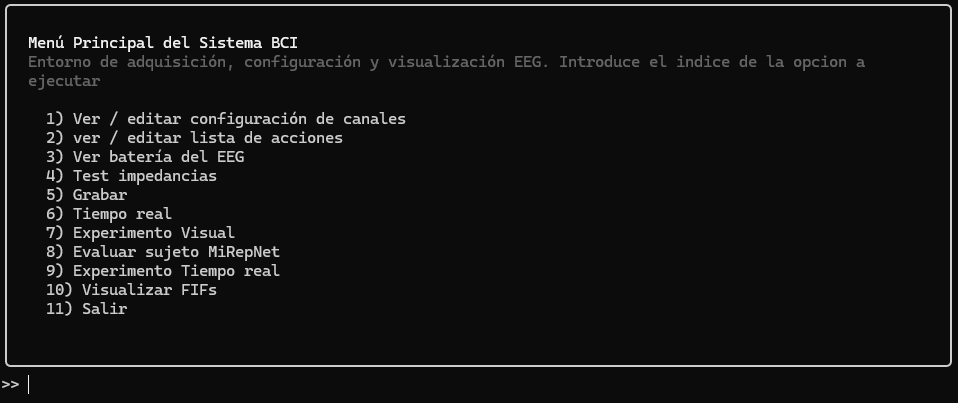
\includegraphics[width=1\textwidth]{Imagenes/Bitmap/menu_principal_app.png}
    \caption{Menú principal de la aplicación BCI.}
    \label{fig:menuPrincipal}
\end{figure}

Las opciones que se visualizan en el menú son las siguientes:
\begin{enumerate}
    \item Ver / editar configuración de canales.
    \item Ver / editar lista de acciones.
    \item Ver batería del EEG.
    \item Test de impedancias.
    \item Grabación manual.
    \item Visualización en tiempo real.
    \item Experimento Visual con protocolo.
    \item Evaluar sujeto con el modelo MiRepNet.
    \item Experimento en Tiempo Real.
    \item Visualizar grabaciones (\textit{FIF}).
\end{enumerate}

\subsection{Configuración del dispositivo EEG}
\label{subsec:configuracionCasco}

Antes de realizar cualquier tipo de grabación o experimento en tiempo real es estrictamente necesario configurar correctamente el dispositivo EEG.Esta sección agrupa las herramientas destinadas a verificar y ajustar el estado de los electrodos y la batería del dispositivo así como también la lista de acciones para la grabación manual.

\subsubsection{Configuración de electrodos}
\label{subsubsec:configuracionElectrodos}

Esta sección permite visualizar y editar la configuración de los canales del casco EEG. Para cada electrodo es posible especificar si está activo o inactivo, asignarle un nombre de canal y una posición estándar según el sistema internacional 10–20, así como designar qué electrodo actúa como BIAS. A diferencia del sistema de configuración de la aplicación BrainAccess, el módulo desarrollado incorpora la posibilidad de guardar y gestionar múltiples configuraciones de forma persistente. Esto resulta especialmente útil cuando se trabaja con distintas disposiciones de electrodos, ya que permite alternar entre configuraciones de forma sencilla sin necesidad de reconfigurar el sistema manualmente en cada sesión. Las configuraciones se almacenan en disco y se cargan automáticamente al iniciar la aplicación (véase Figura~\ref{fig:configuracionElectrodos}).

\begin{figure}[h]
    \centering
    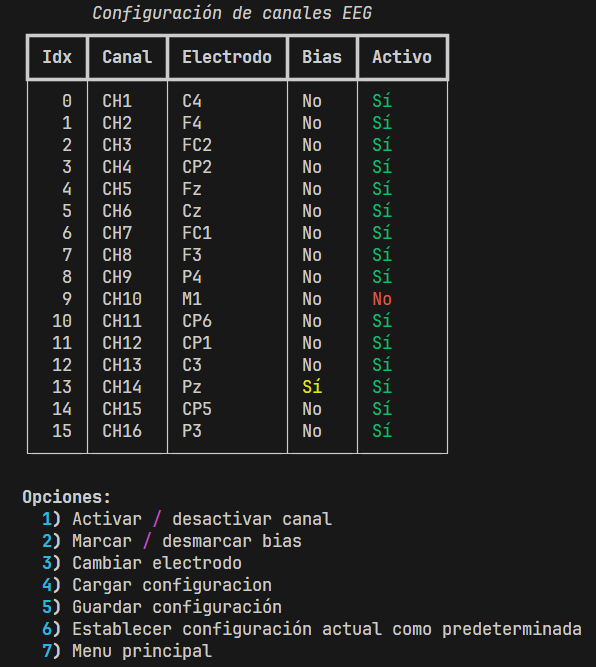
\includegraphics[width=0.7\textwidth]{Imagenes/Bitmap/configuracion_electrodos_app.png}
    \caption{Configuración de electrodos en la aplicación con la tabla de electrodos, sus posiciones, y el menú de opciones.}
    \label{fig:configuracionElectrodos}
\end{figure}

\subsubsection{Configuración de acciones}
\label{subsubsec:configuracionAcciones}

Permite definir las acciones de imaginación motora que se utilizarán durante los experimentos. Cada acción se asocia a una etiqueta y un identificador numérico que actúan como marcadores en los ficheros de grabación. La lista de acciones estará disponible durante las grabaciones manuales, siendo el usuario quien indica mediante comandos el inicio de una determinada acción o la ocurrencia de un evento concreto (véase Figura~\ref{fig:configuracionAcciones}).

\begin{figure}[h]
    \centering
    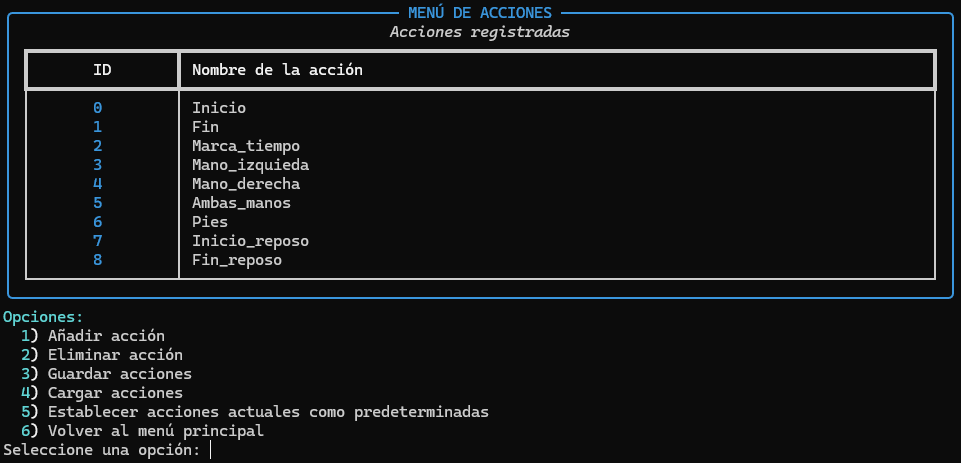
\includegraphics[width=1\textwidth]{Imagenes/Bitmap/configuracion_acciones_app.png}
    \caption{Configuración de acciones en la aplicación con la tabla de acciones, sus índices, y el menú de opciones.}
    \label{fig:configuracionAcciones}
\end{figure}

\subsubsection{Ver batería del EEG}
\label{subsubsec:verBateria}

Muestra el nivel de batería actual del dispositivo EEG. Resulta útil comprobar este valor antes de iniciar sesiones largas de grabación para evitar interrupciones (véase Figura~\ref{fig:visualizacionBateria}).


\begin{figure}[h]
    \centering
    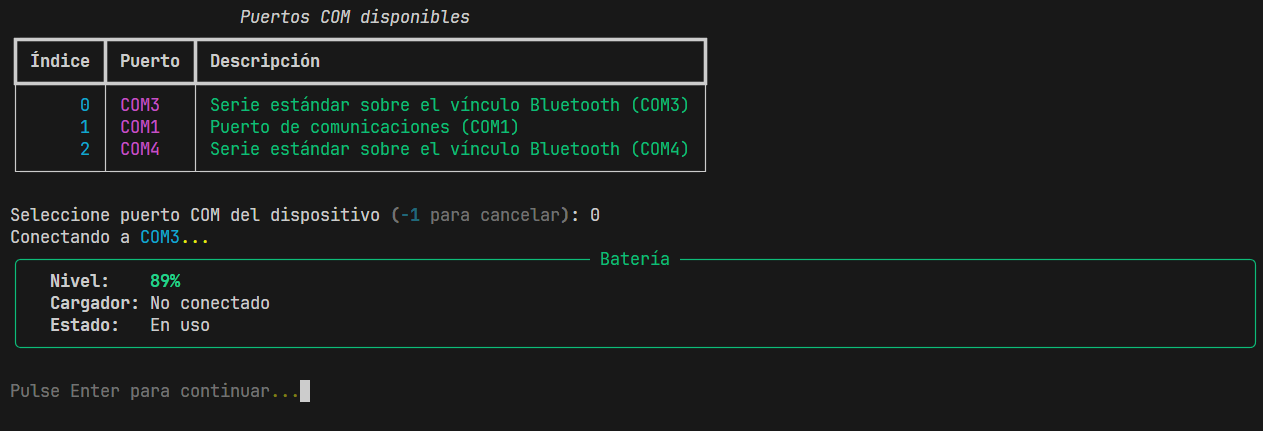
\includegraphics[width=1\textwidth]{Imagenes/Bitmap/conexion_bluethooth_y_bateria_app.png}
    \caption{Visualización del estado de la batería del dispositivo EEG.}
    \label{fig:visualizacionBateria}
\end{figure}

\subsubsection{Test de impedancias}
\label{subsubsec:testImpedancias}

Permite realizar una medición interactiva de la impedancia de los electrodos. Una impedancia elevada refleja un contacto deficiente entre el electrodo y el cuero cabelludo, lo que degrada la calidad de la señal adquirida y puede introducir ruido de baja frecuencia, artefactos o distorsiones en determinadas bandas de frecuencia. Este módulo guía al usuario a través de la comprobación de cada canal activo, permitiendo verificar que todos los electrodos estén correctamente posicionados y que sus valores de impedancia se encuentren dentro del rango aceptable antes de iniciar una grabación o experimento (véase Figura~\ref{fig:medicionImpedancias}). Además, se incluye una representación gráfica en 2D del cuero cabelludo con la disposición de los electrodos activos, en la que cada canal se colorea en función de su nivel de impedancia, facilitando la identificación visual e inmediata de los electrodos problemáticos sin necesidad de consultar un dibujo de posiciones y nombres (véase Figura~\ref{fig:visualizacionImpedancias}).

\begin{figure}[h]
    \centering
    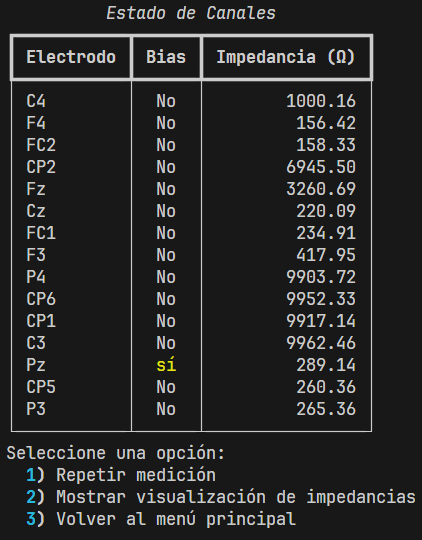
\includegraphics[width=0.5\textwidth]{Imagenes/Bitmap/medicion_impedancias_app.png}
    \caption{Ejemplo de medición de impedancias en la aplicación con la tabla de electrodos, sus posiciones,su impedancia medida en k$\Omega$, y el menú de opciones.}
    \label{fig:medicionImpedancias}
\end{figure}

\begin{figure}[h]
    \centering
    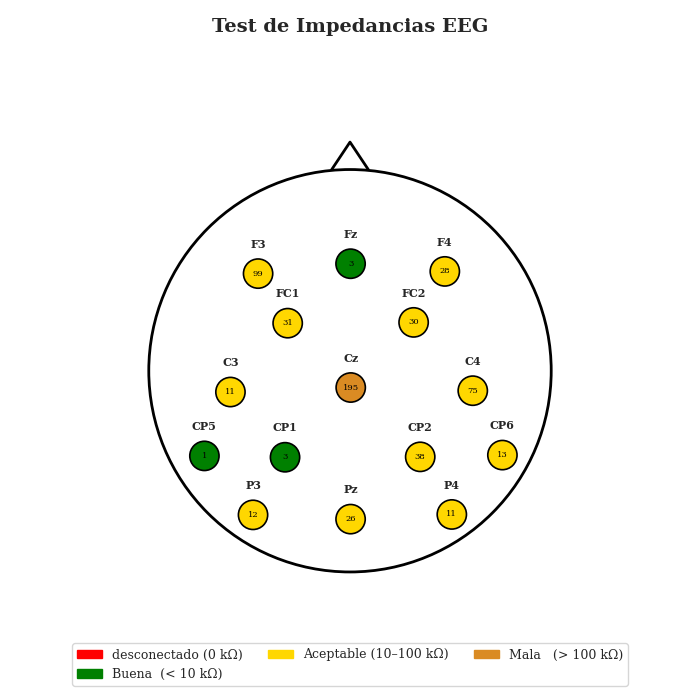
\includegraphics[width=0.9\textwidth]{Imagenes/Bitmap/visualizar_impedancias_app.png}
    \caption{Visualización de impedancias en la aplicación mediante un gráfico 2D: en verde los electrodos con impedancia baja ($<$10~k$\Omega$), en amarillo de 10 a 100~k$\Omega$, en naranja superior a 100~k$\Omega$ y en rojo los que no están haciendo contacto (0~k$\Omega$).}
    \label{fig:visualizacionImpedancias}
\end{figure}

\subsection{Grabación Manual}
\label{subsec:grabacionManual}

La grabación manual permite iniciar y detener la adquisición de señales EEG de forma libre, sin seguir un protocolo de estimulación predefinido. El usuario controla en todo momento qué acción se está etiquetando mediante los comandos de teclado disponibles.

\subsubsection{Control de acciones}
\label{subsubsec:controlAcciones}

\begin{figure}[h]
    \centering
    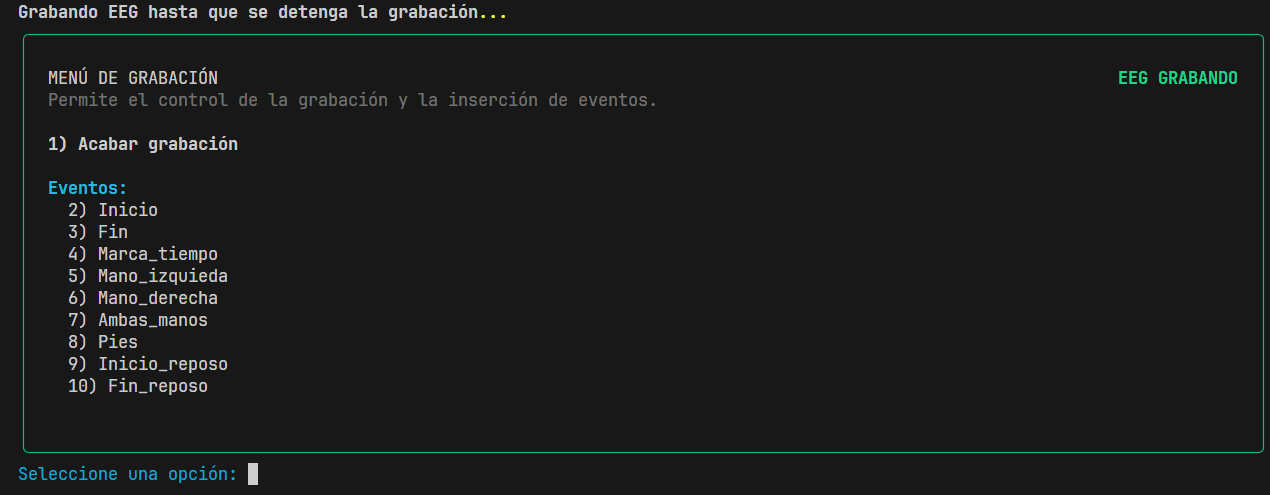
\includegraphics[width=1\textwidth]{Imagenes/Bitmap/menu_grabacion_manual_app.png}
    \caption{Menú de la grabación manual con todas las acciones cargadas y opción de terminar grabación.}
    \label{fig:menuGrabacionManual}
\end{figure}

Durante la grabación (véase Figura~\ref{fig:menuGrabacionManual}), el usuario puede seleccionar la acción activa en cada instante pulsando la tecla correspondiente. El sistema inserta el marcador de evento apropiado en la señal, de modo que cada segmento queda correctamente etiquetado para su posterior análisis.

\subsection{Visualización en tiempo real}
\label{subsec:visualizacionTiempoReal}

Este módulo se encarga de la adquisición y visualización en tiempo real de la señal EEG. Aunque se trata de una funcionalidad de carácter básico, ha resultado de gran utilidad para inspeccionar visualmente la señal del sujeto y observar el efecto de artefactos frecuentes como los producidos por parpadeos, habla o ruido muscular, permitiendo valorar la calidad de la adquisición antes de iniciar cualquier experimento.

\subsection{Experimento Visual}
\label{subsec:experimentoVisual}

El Experimento Visual es el módulo encargado de la adquisición guiada de señales EEG mediante un protocolo estructurado de estimulación visual y auditiva. Su objetivo es obtener grabaciones con una estructura temporal bien definida y de mayor calidad que la grabación manual, eliminando fuentes de contaminación como el ruido asociado a la comunicación oral o la presencia de estímulos impredecibles. Adicionalmente, el módulo incorpora una opción de servidor TCP que permite visualizar en tiempo real las lecturas EEG durante el transcurso de la grabación, facilitando que un supervisor pueda monitorizar la calidad de la señal y verificar que la adquisición se está realizando correctamente. Esta modalidad constituye la principal vía de adquisición de datos de sujetos para el entrenamiento y evaluación del sistema.

\subsubsection{Funcionamiento de grabaciones}
\label{subsubsec:funcionamientoGrabaciones}

Durante el experimento, se presenta al sujeto una secuencia de estímulos visuales y sonoros que indican los sucesivos pasos que componen el protocolo: qué acción de imaginación motora debe realizar, cuándo el sujeto puede descansar y cuándo debe centrar la atención. Las señales EEG se registran de forma continua y los eventos quedan marcados como eventos correspondientes a cada acción en la grabación resultante. Al finalizar, la grabación se almacena en formato \textit{FIF}, compatible con la librería MNE para su posterior utilización.

\subsubsection{Protocolo}
\label{subsubsec:protocoloExperimento}

El protocolo define la estructura temporal del experimento: el número de repeticiones de imaginación motora (epochs) por clase, y que clases aparecerán (mano izquierda, mano derecha y pies), la duración de los periodos de imaginación motora, los intervalos de descanso entre epochs y las instrucciones presentadas al sujeto durante cada fase. Todos estos parámetros son configurables, lo que permite adaptar el experimento de forma flexible a las necesidades específicas de cada sesión o participante.

\subsection{Evaluación de sujetos con el modelo MiRepNet}
\label{subsec:evaluacionMiRepNet}

Este módulo automatiza la evaluación del rendimiento del sistema sobre las grabaciones de un sujeto. El usuario puede seleccionar, para un sujeto determinado, las grabaciones concretas que desea incluir en la evaluación, lo que permite analizar el rendimiento y la precisión (\textit{accuracy}) obtenidos en cada conjunto e identificar qué condiciones o sesiones arrojan mejores resultados. Para ello, se aplica el pipeline completo de preprocesado, que incorpora una etapa de detección y descarte de épocas ruidosas, se realiza el ajuste fino (\textit{fine-tuning}) del modelo predictor MiRepNet sobre los datos del sujeto y se calculan métricas de clasificación mediante validación cruzada, lo que facilita la comparación del desempeño entre distintos sujetos y sesiones. Una vez finalizada la evaluación, los resultados se presentan de forma visual mediante un conjunto de gráficas que incluyen la evolución de la precisión y del \textit{learning rate} a lo largo del entrenamiento, la matriz de confusión, un diagrama de cajas y bigotes y un diagrama de barras con la \textit{precision}, \textit{recall} y \textit{accuracy} desglosados por clase, proporcionando una visión completa del comportamiento del modelo (véase Figura~\ref{fig:modeloGraficoFinetune} y Figura~\ref{fig:modeloGraficoMatriz}).
\begin{figure}[h]
    \centering
    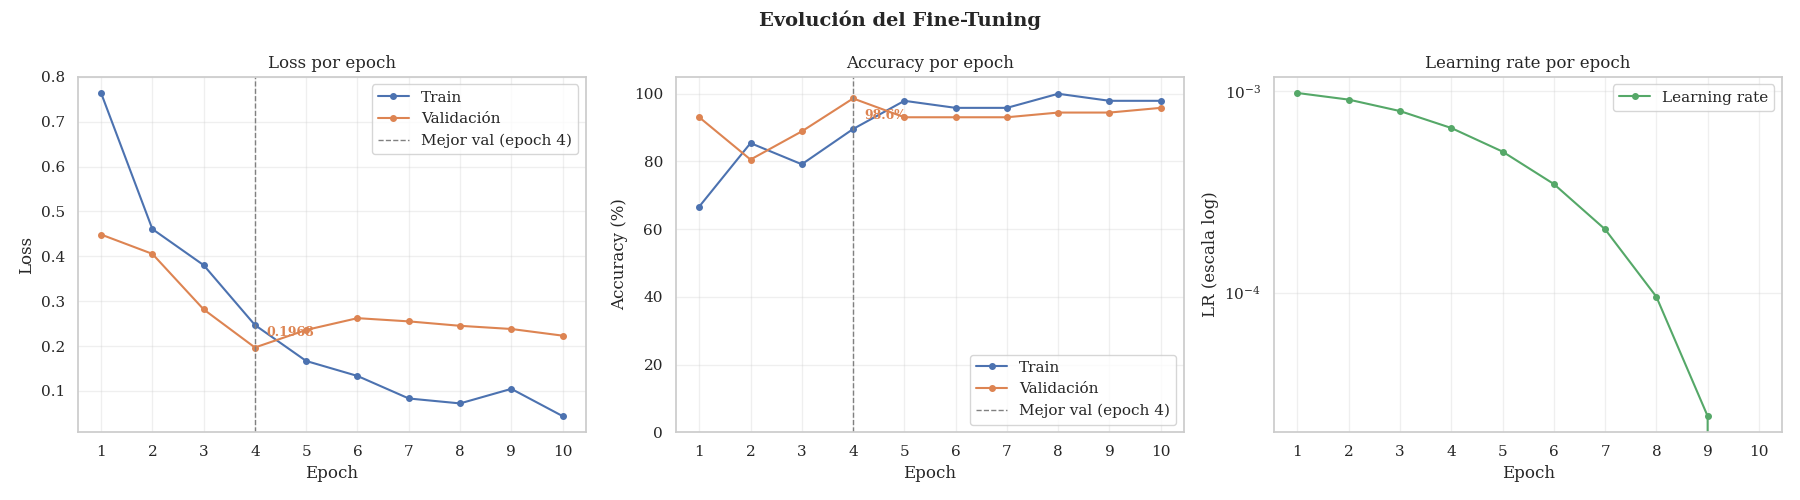
\includegraphics[width=1\textwidth]{Imagenes/Bitmap/modelo_grafico_1.png}
    \caption{Gráficos del resultado de evaluación con accuracy, loss y learning rate por epoch.}
    \label{fig:modeloGraficoFinetune}
\end{figure}

\begin{figure}[h]
    \centering
    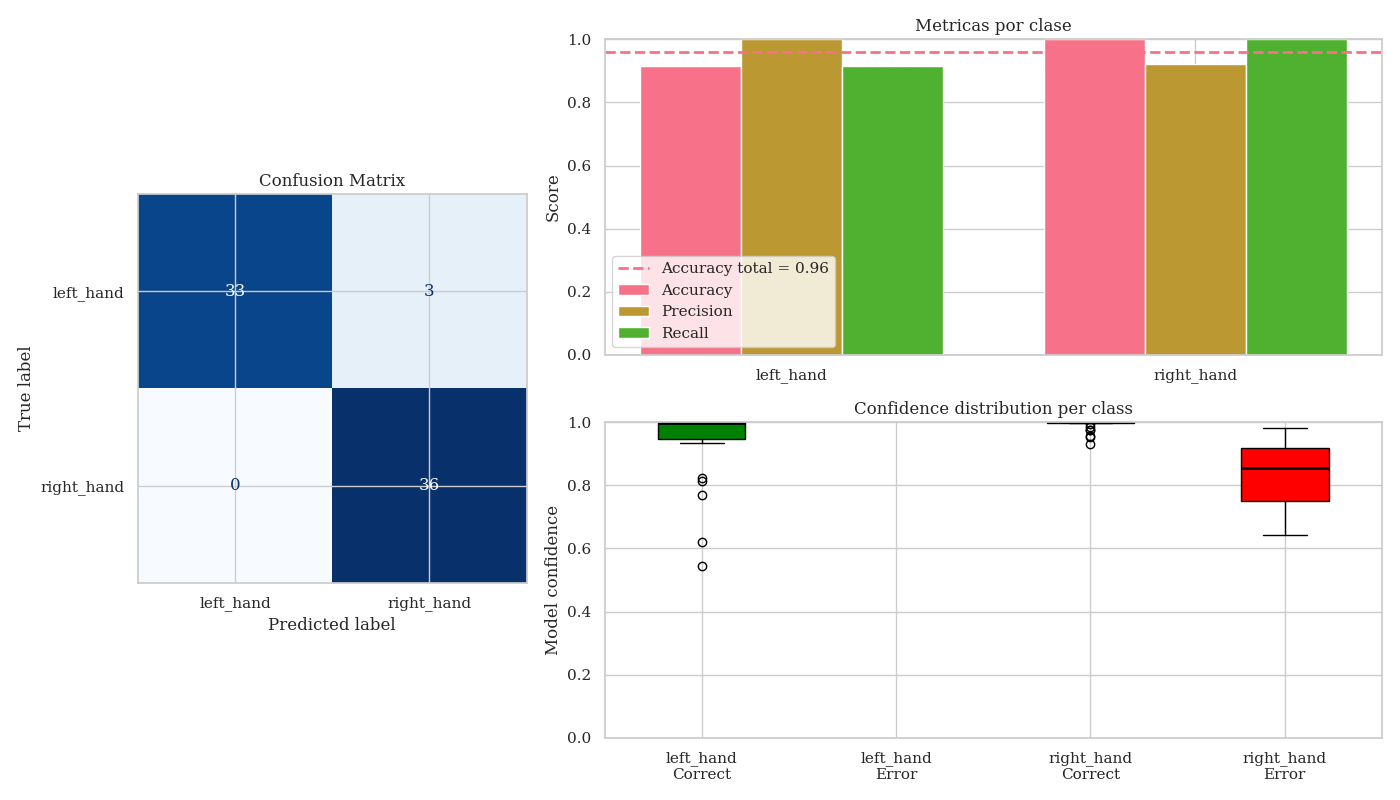
\includegraphics[width=1\textwidth]{Imagenes/Bitmap/modelo_grafico_2.png}
    \caption{Matriz de confusión del resultado del fine-tuning y validación del modelo MiRepNet, gráfico con accuracy, precision y recall, y diagrama de bigotes o cajas.}
    \label{fig:modeloGraficoMatriz}
\end{figure}

\subsection{Experimento en Tiempo Real}
\label{subsec:experimentoTiempoReal}

El módulo de Experimento en Tiempo Real constituye la implementación completa del pipeline de interfaz cerebro-computador, integrando de las etapas de adquisición de señal EEG, filtrado, normalización e inferencia del modelo predictor. El resultado es un sistema capaz de traducir la imaginación motora del sujeto en acciones concretas sobre un entorno de benchmarking o videojuego. Para garantizar un rendimiento adecuado, el módulo incorpora una fase previa de entrenamiento idéntica a la del Experimento Visual, que permite ajustar el modelo predictor a las características individuales del sujeto antes de iniciar la sesión en tiempo real.

\subsubsection{Training}
\label{subsubsec:training}

Antes de iniciar la fase en tiempo real, el módulo lleva a cabo una fase previa de entrenamiento, imprescindible para adaptar el modelo predictor a las características individuales del sujeto. Durante esta fase, se realiza una grabación siguiendo el mismo protocolo parametrizable del Experimento Visual, adquiriendo así los datos necesarios para realizar el ajuste fino \textit{fine-tuning} del modelo antes de lanzar la sesión en tiempo real.

\subsubsection{Juegos y benchmarks BCI}
\label{subsubsec:juegosBCI}

Una vez finalizada la fase de entrenamiento, el sujeto puede interactuar con los entornos BCI desarrollados, que pueden tomar la forma de aplicaciones de benchmarking, orientadas a la evaluación objetiva del rendimiento del sistema, o de entornos de juego, orientados a una experiencia más inmersiva e intuitiva para el usuario. Durante la sesión, el modelo genera de forma continua un elevado número de predicciones que son procesadas y convertidas en acciones mediante filtros de decisión. Adicionalmente, los entornos de juego incorporan mecanismos de asistencia que facilitan la interacción del usuario con el entorno, compensando la variabilidad inherente a la señal EEG y mejorando la experiencia de uso.

\subsection{Visualizador de grabaciones}
\label{subsec:visualizadorGrabaciones}

El visualizador de grabaciones permite revisar los ficheros \textit{FIF} generados durante los experimentos. Muestra las señales EEG de cada canal en el dominio temporal junto con los marcadores de eventos asociados, facilitando la inspección visual de la calidad de las grabaciones y la detección de artefactos (véase Figura~\ref{fig:visualizacionFIF}).

\begin{figure}[h]
    \centering
    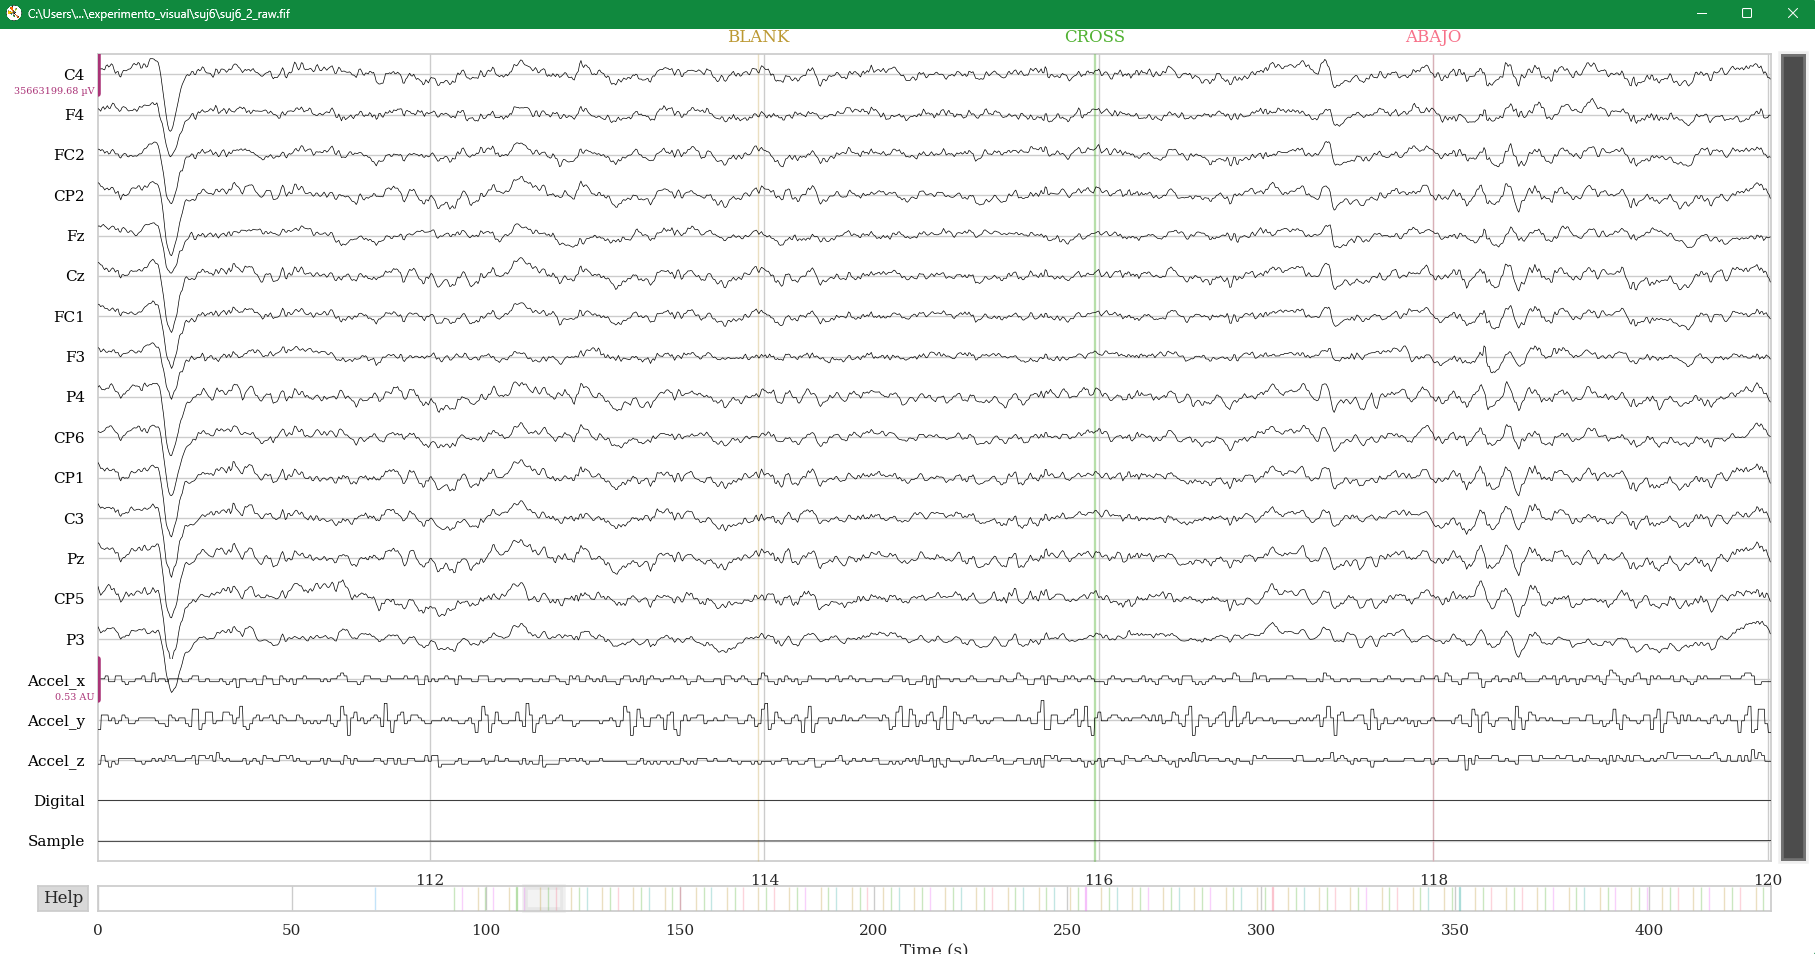
\includegraphics[width=1\textwidth]{Imagenes/Bitmap/visualizacion_fif_app.png}
    \caption{Visualización de grabaciones en formato \textit{FIF} con la señal EEG de cada canal y acelerómetros y los eventos marcados.}
    \label{fig:visualizacionFIF}
\end{figure}

\subsection{Implementación}
\label{subsec:implementacion}
